% Definition of circles and square
\def\firstcircle{(0,0) circle (1.5cm)}
\def\secondcircle{(0:2cm) circle (1.5cm)}
\def\firstsquare{(-1.6,-1.6) rectangle (1.6,1.6)}

% Set colors
\colorlet{circle edge}{blue!50}
\colorlet{circle area}{blue!20}
\colorlet{rectangle edge}{blue!50}
\colorlet{rectangle area}{blue!20}

\tikzset{filled/.style={fill=circle area, draw=circle edge, thick},
    outline/.style={draw=circle edge, thick}}
\setlength{\parskip}{5mm}


\begin{tabular}{p{2.25in} p{2.25in} p{2.25in}}

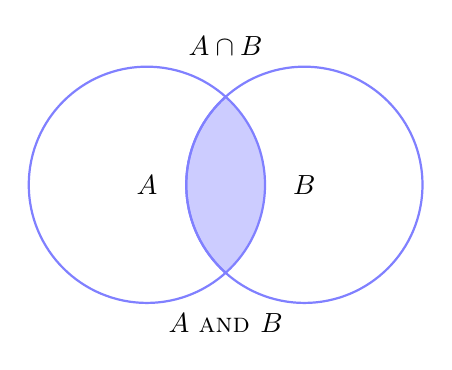
\begin{tikzpicture}

	\begin{scope}
        \clip \firstcircle;
        \fill[filled] \secondcircle;
    \end{scope}

    \draw[outline] \firstcircle node {$A$};
    \draw[outline] \secondcircle node {$B$};
    \node[anchor=south] at (current bounding box.north) {$A \cap B$};
	\node[anchor=north] at (current bounding box.south) {$A$ \sc{and} $B$};

\end{tikzpicture}

&

% Set A or B
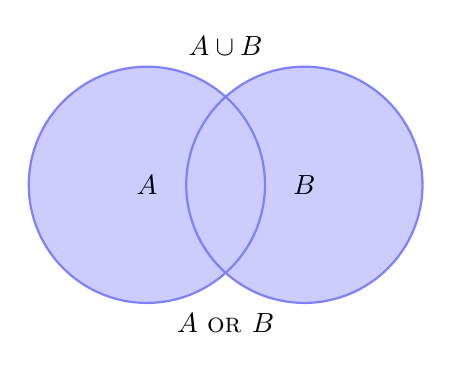
\begin{tikzpicture}

    \draw[filled] \firstcircle node {$A$}
                  \secondcircle node {$B$};
    \node[anchor=south] at (current bounding box.north) {$A \cup B$};
	\node[anchor=north] at (current bounding box.south) {$A$ \sc{or} $B$};

\end{tikzpicture}

&

% NOT A

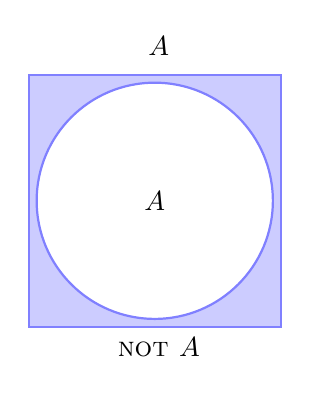
\begin{tikzpicture}

	\filldraw[blue!20,even odd rule] \firstsquare \firstcircle;
	\draw[outline] \firstcircle node{$A$};
	\draw[outline] \firstsquare node{};
	\node[anchor=south] at (current bounding box.north) {$\thicksim A$};
	\node[anchor=north] at (current bounding box.south) {\sc{not} $A$};

\end{tikzpicture}

\\

\end{tabular}
